% !TeX spellcheck = en_US
\documentclass{article}
\usepackage{pacco}
	\makeindex
\begin{document}
	\tableofcontents
\section{Basics of probability}
We start with the probability triplet: $(\Omega,\mathcal{H},\mathbbm{P})$ 
Here $\Omega$ is the set of sample space, $\mathcal{H}$ is the $\sigma$-algebra built upon $\Omega$ and $\pr$ is the probability measure. Since $\pr$ is a measure, it will take values in $\R$. \\
We are interested in probability measure, which means:
\begin{itemize}
	\item $\pr$ is a \textbf{finite measure} and $\pr(\Omega)=1$;
	\item $\omega \in\Omega$ will be called \textbf{outcomes}.
\end{itemize}
So consider the example of the roll of the die. If we roll it, 
\[\Omega=\underbrace{\left\{1,2,3,4,5,6\right\}}_{\text{outcomes}}\]
And if we considere the elements $A\in\mathcal{H}$ (which will be subsets of $\Omega$) will be called \textbf{events}.\par We want to quantify the possibility that the event $A$ occurs: we want to measure, through $\pr$, the set $A$: from a measure theory point of view, it's only sets in the $\sigma$-algebra. \\The probability measure has the following properties:
\begin{itemize}
	\item $\pr(\Omega)=1,\quad\pr(\emptyset)=0$
	\item \textbf{monotonicity of $\pr$}: take 2 events $H,K\in\mathcal{H}$ such that $H\subset K$. Then $\pr(H)\leqslant\pr(K)$\footnote{note that the notation is loose since we have proper subset on one side and leq on the other side. But this is not much of a problem, since i will kill myself very soon.}.
	\item \textbf{finite additivity}: take $H,K\in\mathcal{H}$ such that $H\cap K=\emptyset$. The $\pr(H\cup K)=\pr(H)+\pr(K)$;
	\item \textbf{countable additivity}: this requires that we consider collection of events. We denote them in this way:
	\[\left(H_n\right)_{n\in\N}\subset\mathcal{H}\] with $\N=\{0,1,2,3,\ldots\}$ and $\N^\star=\{1,2,3,4,\ldots\}$ such that they are disjoint pairwise (except identical pairs). Then
	\[\pr\left(\bigcup_nH_n\right)=\sum_n\pr\left(H_n\right)\]
	\item \textbf{Boole inequality (sub-additivity)}: if we have a collection $\left(H_n\right)_{n\in\N}\subset\mathcal{H}$ (not necessarily disjoint) then $$\pr\left(\bigcup_nH_n\right)\leqslant\sum_n\pr\left(H_n\right)$$ 
	\item \textbf{sequential continuity}: consider the sequence $\left(H_n\right)_{n\in\N}\subset\mathcal{H}$ such that $H_n\nearrow H\in\mathcal{H}$ ($H_n$ is an increasing sequence of numbers that has $H$ as limit) then $\pr(H_n)\nearrow\pr(H)$. Moreover, if $\left(F_n\right)_{n\in\N}\subset\mathcal{H}$ such that $F_n\searrow F\in\mathcal{H}$ then $\pr(F_n)\searrow\pr(F)$. The second property is actually true because $\pr$ is finite (it is not true for infinite measures). 
\end{itemize}
In measure theory we encounter the concept of \textbf{negligible sets}: these are sets of measure zero or non measurable sets included in measure zero sets. In probability theory, sets are \textbf{events}: so we have negligible events (events with probability 0 or non measurable events included in events with probability 0). Analogously, in measure theory a property which holds \textbf{almost everywhere} is allowed not to hold on negligible sets. In probability theory a property which holds \textbf{almost surely} is allowed not to hold on negligible events.
We also have, in measure theory, \textit{measurable functions} that in probability theory are \textbf{random variables}.
\subsection{Random variables}
Consider a measurable space $(E,\mathcal{E})$. 
\begin{definition}
	A mapping $X:\Omega\rightarrow E$ is called \enf{random variable taking values in $E$} if $X$ is measurable relative to $\mathcal{H}$ and $\mathcal{E}$.
\end{definition}
What does it mean\footnote{who asked}? The inverse image of the set $A$ through $X$ ($X^{-1}A$) with $A\in \mathcal{E}$ is actually the set of the $\omega$s such that $X(\omega)$ arrives to $A$. So
\[X^{-1}A=\left\{\omega\in\Omega:X(\omega)\in A\right\}=\left\{X\in A\right\}\] so that $X^{-1}A$ is an event for all $A$ in $\mathcal{E}$.
\begin{figure}[H]
	\centering
	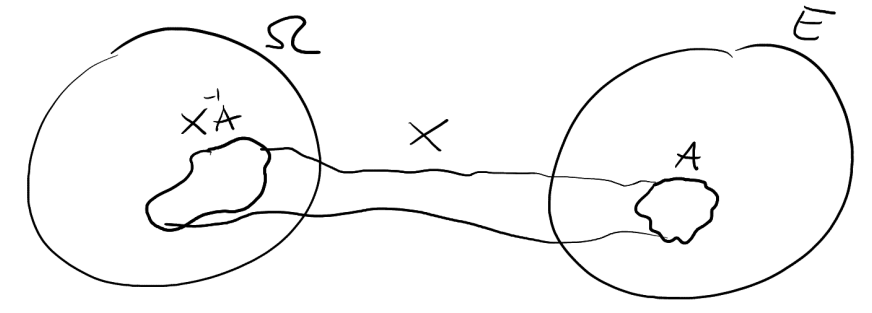
\includegraphics[width=0.7\linewidth]{screenshot001}
	\caption{this is an early reminder of the fact that I will take my own life very soon.}
	\label{fig:screenshot001}
\end{figure}
So if $X^{-1}A$ is measurable by $\pr$ then it is in $\mathcal{H}$: otherwise it is not in $\mathcal{H}$. So \[\pr(X^{-1}A)=\pr\left(\left\{\omega\in\Omega:X(\omega)\in A\right\}\right).\] The message is that I am interested/able to evaluate $\pr$ over the set only if what I am evaluating is indeed an event (which means: it belongs to $\mathcal{H}$\footnote{il lettore più arguto avrà notato che, a questo punto, il dio è ormai irrimediabilmente cane.}). If something is not in $\mathcal{H}$ get it off my fucking face man and kill yourself NOW\footnote{
		
\includegraphics[width=0.05\linewidth]{screenshot002}
}. This is the only restriction for a random variable. $E$ can be whatever we need it to be: a graph, a tree, your mom being absolutely \censor{torn apart} by me. But most of the times, we have $E=\R$ or $E=\R^d$ with respectively $\mathcal{E}=\mathcal{B}\footnote{Borel $\sigma$-algebra}(\R)=\mathcal{B}_\R$ and $\mathcal{B}_{\R^d}$.
\begin{remark}
	The simplest random variables are indicator functions of events.
	Example: take $H\in\mathcal{H}$. Define the function
	\begin{align*}
		\indi_H&:\Omega\rightarrow\R\\
		\indi_H(\omega)&=\begin{cases}
			0 &\omega\not\in H\\
			1 &\omega\in H
		\end{cases}
	\end{align*}
\end{remark}
\begin{remark}
	A random variable is said to be \enf{simple} if it takes only finitely many values in $\R^d$.
\end{remark}
\begin{remark}
	A random variable is said to be \enf{discrete} if it takes only countably many values.
\end{remark}
\begin{definition}
	\enf{Distribution of a random variable}. Let $X$ be a random variable taking values in $(E,\mathcal{E})$ and let $\mu$ be the image of $\pr$ under $X$, that is,
	\[\mu(A)=\pr(X^{-1}A)=\pr(X\in A)=\pr\circ X^{-1}(A)\footnote{you would know this if you knew fucking measure theory I guess},\;A\in\mathcal{E}.\] Then $\mu$ is a probability measyre on $(E,\mathcal{E})$ and it is called \textbf{distribution of X}.
\end{definition}
So we map, by means of $X$, sets belonging to $\mathcal{E}$ into $\mathcal{H}$ and then evaluates this sets by means of the measure $\pr$. This is what we mean when we say that distributions are ultimately built with the probability measure and the random variable. Distribution is itself a measure!
\begin{remark}
	You should remember (LOL) that when we want to specify a measure on a $\sigma$-algebra, it's enough to do it on a \textit{p-system}\footnote{a p-system is a simpler object than a $\sigma$-algebra: it is simply a collection of sets closed under intersection} generating that $\sigma$ algebra: by means of the monotone class theorem we are then able to extend the measure to the $\sigma$-algebra. \\
	This means that to specity $\mu$ it is enough to specify it on a \textit{p-system} which generates $\mathcal{E}$. For example, consider $E=\overline{\R}, \mathcal{E}=\mathcal{B}_{\overline{\R}}$. Consider the collection of sets $[-\infty,x],\;x\in\R$ which is of course a p-system because it is closed under intersection. Moreover, this shit generates the Borel sigma algebra on $\overline{\R}$. \\If we want to define a distribution, that is a measure, it is enough to define it on this p-system. Imagine that we apply our distribution measure to one set of this p-system
	\[c(x)\footnote{because it is a function of $x$}=\mu\left([-\infty,x]\right)=\pr(X\leq x),\qquad x\in\R\] by the monotone class theorem. So we have now specified the measure on the p-system. The part $\pr(X\leq x)$ reminds us of the undergraduate times\footnote{I already wanted to kill myself at that time.}: it is a distribution function! This is what our professor did implicitly to avoid using measure theory\footnote{I have noticed that my life has not benefited in ANY form since I was introduced to measure theory.}
\end{remark}
\subsection{Functions of random variables}
Consider $X$, a random variable taking values in $(E,\mathcal{E})$ and consider further a measurable space $(F,\mathcal{F})$. Let $f:E\rightarrow F$ be a measurable function relative to $\mathcal{E}$ and $\mathcal{F}$\footnote{This basically means that this bitch won't do anything evil. The whole point of measure theory, $\sigma$ algebras and all other shit is to ensure everything behaves.}. This function should me measurable by means of $\pr$, otherwise we couldn't do anything useful with it. Consider the composition
\[Y=f\circ X\qquad\text{such that}\;Y(\omega)=f\circ X(\omega)=f\big(X(\omega)\big),\;\omega\in\Omega.\]
This composition is a random variable taking values in $(F,\mathcal{F})$
\end{document}